%%%%%%%%%%%%%%%%%%%%%%%%%%%%%%%%%%%%%%%%%%%%%%%%%%%%%%%%%%%%%%%%%%%%%%%%%%%%%%%%%%%%%%%%%%%%%%%%%
%
% Document:      DM  product tree
%
%%%%%%%%%%%%%%%%%%%%%%%%%%%%%%%%%%%%%%%%%%%%%%%%%%%%%%%%%%%%%%%%%%%%%%%%%%%%%%
\documentclass{article}
\usepackage{times,layouts}
\usepackage{tikz,hyperref,amsmath}
\usetikzlibrary{positioning,arrows,shapes,decorations.shapes,shapes.arrows}
\usetikzlibrary{backgrounds,calc}
\usepackage[paperwidth=20.6cm,paperheight=198.6cm,
left=-2mm,top=3mm,bottom=0mm,right=0mm,
noheadfoot,marginparwidth=0pt,includemp=false,
textwidth=30cm,textheight=50mm]{geometry}
\newcommand\showpage{%
\setlayoutscale{0.5}\setlabelfont{\tiny}\printheadingsfalse\printparametersfalse
\currentpage\pagedesign}
\hypersetup{pdftitle={DM products }, pdfsubject={Diagram illustrating the
products in LSST DM }, pdfauthor={ William O'Mullane}}
\tikzstyle{tbox}=[rectangle,text centered, text width=30mm]
\tikzstyle{wbbox}=[rectangle, rounded corners=3pt, draw=black, top color=blue!50!white, bottom color=white, very thick, minimum height=12mm, inner sep=2pt, text centered, text width=30mm]
\tikzstyle{pbox}=[rectangle, rounded corners=3pt, draw=black, top color=yellow!50!white, bottom color=white, very thick, minimum height=28pt, inner sep=2pt, text centered, text width=35mm]
\tikzstyle{pline}=[-, thick]\begin{document}
\begin{tikzpicture}[node distance=0mm]
\node (DM) [wbbox]{\textbf{Data Management}};
\node (DAC) [pbox,right=15mm of DM] {{\tiny \color{gray}.} \newline
\textbf{Data Access Center}
 };
 \draw[pline] (DM.east) -| ++(0.4,0)  |- (DAC.west);
 \node (BULKD) [pbox,right=15mm of DAC] {\textbf{Bulk Distrib}
 };
 \draw[pline] (DAC.east) -| ++(0.4,0)  |- (BULKD.west);
 \node (DACPROP) [pbox,below=4pt of BULKD] {\textbf{Proposal Manager}
 };
 \draw[pline] (DAC.east) -| ++(0.4,0)  |- (DACPROP.west);
 \node (DACRM) [pbox,below=4pt of DACPROP] {\textbf{Resource Manager}
 };
 \draw[pline] (DAC.east) -| ++(0.4,0)  |- (DACRM.west);
 \node (DBB) [pbox,below=68pt of DAC] {{\tiny \color{gray}.} \newline
\textbf{Data Backbone}
 };
 \draw[pline] (DM.east) -| ++(0.4,0)  |- (DBB.west);
 \node (BUTLER) [pbox,right=15mm of DBB] {{\tiny \color{gray}1.02C.06.02.01} \newline
\textbf{Data Butler Client}
 };
\node (BUTLERpkg) [tbox,below=3mm of BUTLER.north] {{\tiny \color{gray} \begin{verbatim} daf_persistence/db/daf_fmt_* \end{verbatim} }  };
 \draw[pline] (DBB.east) -| ++(0.4,0)  |- (BUTLER.west);
 \node (DTR) [pbox,below=4pt of BUTLER] {\textbf{Transport/Repl}
 };
 \draw[pline] (DBB.east) -| ++(0.4,0)  |- (DTR.west);
 \node (SCICATAR) [pbox,below=4pt of DTR] {{\tiny \color{gray}.} \newline
\textbf{Science Cat Archive}
 };
 \draw[pline] (DBB.east) -| ++(0.4,0)  |- (SCICATAR.west);
 \node (QSERV) [pbox,right=15mm of SCICATAR] {{\tiny \color{gray}1.02C.06.02.03} \newline
\textbf{Qserv DBMS}
 };
\node (QSERVpkg) [tbox,below=3mm of QSERV.north] {{\tiny \color{gray} \begin{verbatim} qserv/partition/scisql \end{verbatim} }  };
 \draw[pline] (SCICATAR.east) -| ++(0.4,0)  |- (QSERV.west);
 \node (SCICATDB) [pbox,below=4pt of QSERV] {{\tiny \color{gray}.} \newline
\textbf{Science Cat DBs}
 };
 \draw[pline] (SCICATAR.east) -| ++(0.4,0)  |- (SCICATDB.west);
 \node (SCIIMGAR) [pbox,below=34pt of SCICATAR] {{\tiny \color{gray}.} \newline
\textbf{Science Img Archive}
 };
 \draw[pline] (DBB.east) -| ++(0.4,0)  |- (SCIIMGAR.west);
 \node (GMDS) [pbox,right=15mm of SCIIMGAR] {{\tiny \color{gray}1.02C.06.02.05} \newline
\textbf{Global Metadata}
 };
 \draw[pline] (SCIIMGAR.east) -| ++(0.4,0)  |- (GMDS.west);
 \node (PRVDB) [pbox,below=4pt of GMDS] {{\tiny \color{gray}1.02C.06.01.01} \newline
\textbf{Provenance DB}
 };
 \draw[pline] (SCIIMGAR.east) -| ++(0.4,0)  |- (PRVDB.west);
 \node (DEVEL) [pbox,below=204pt of DBB] {{\tiny \color{gray}.} \newline
\textbf{Developer services}
 };
 \draw[pline] (DM.east) -| ++(0.4,0)  |- (DEVEL.west);
 \node (BUILD) [pbox,right=15mm of DEVEL] {{\tiny \color{gray}1.02C.10.02.03.01} \newline
\textbf{Build/Unit Test}
 };
\node (BUILDpkg) [tbox,below=3mm of BUILD.north] {{\tiny \color{gray} \begin{verbatim} sconsUtils/base/lsstsw/lsst_build \end{verbatim} }  };
 \draw[pline] (DEVEL.east) -| ++(0.4,0)  |- (BUILD.west);
 \node (COMMS) [pbox,below=4pt of BUILD] {{\tiny \color{gray}1.02C.10.02.03.04} \newline
\textbf{Devel Comm Tools}
 };
 \draw[pline] (DEVEL.east) -| ++(0.4,0)  |- (COMMS.west);
 \node (DOCS) [pbox,below=4pt of COMMS] {{\tiny \color{gray}1.02C.10.02.03.03} \newline
\textbf{Doc Infrastructure}
 };
\node (DOCSpkg) [tbox,below=3mm of DOCS.north] {{\tiny \color{gray} \begin{verbatim} lsst-texmf/templates/lsstDoxygen \end{verbatim} }  };
 \draw[pline] (DEVEL.east) -| ++(0.4,0)  |- (DOCS.west);
 \node (DVCS) [pbox,below=4pt of DOCS] {{\tiny \color{gray}1.02C.10.02.03.01} \newline
\textbf{SW Version Control}
 };
 \draw[pline] (DEVEL.east) -| ++(0.4,0)  |- (DVCS.west);
 \node (ISSUE) [pbox,below=4pt of DVCS] {{\tiny \color{gray}1.02C.10.02.03.05} \newline
\textbf{Issue Tracking}
 };
 \draw[pline] (DEVEL.east) -| ++(0.4,0)  |- (ISSUE.west);
 \node (PKG) [pbox,below=4pt of ISSUE] {{\tiny \color{gray}1.02C.10.02.03.02} \newline
\textbf{Packaging/Distrib}
 };
\node (PKGpkg) [tbox,below=3mm of PKG.north] {{\tiny \color{gray} \begin{verbatim} lsst/shebangtron/lsst_dm_stack_demo \end{verbatim} }  };
 \draw[pline] (DEVEL.east) -| ++(0.4,0)  |- (PKG.west);
 \node (IDM) [pbox,below=170pt of DEVEL] {\textbf{Identity Manager}
 };
 \draw[pline] (DM.east) -| ++(0.4,0)  |- (IDM.west);
 \node (INFRA) [pbox,below=4pt of IDM] {{\tiny \color{gray}.} \newline
\textbf{Infrastructure}
 };
 \draw[pline] (DM.east) -| ++(0.4,0)  |- (INFRA.west);
 \node (BPS) [pbox,right=15mm of INFRA] {\textbf{Batch Proc}
 };
 \draw[pline] (INFRA.east) -| ++(0.4,0)  |- (BPS.west);
 \node (INFRASYS) [pbox,below=4pt of BPS] {\textbf{Infra Systems}
 };
 \draw[pline] (INFRA.east) -| ++(0.4,0)  |- (INFRASYS.west);
 \node (TXF) [pbox,below=4pt of INFRASYS] {{\tiny \color{gray}.} \newline
\textbf{Task Execution}
 };
 \draw[pline] (INFRA.east) -| ++(0.4,0)  |- (TXF.west);
 \node (ACTIVATR) [pbox,right=15mm of TXF] {{\tiny \color{gray}1.02C.06.03} \newline
\textbf{Activator Bases}
 };
 \draw[pline] (TXF.east) -| ++(0.4,0)  |- (ACTIVATR.west);
 \node (CONFIG) [pbox,below=4pt of ACTIVATR] {{\tiny \color{gray}1.02C.06.03} \newline
\textbf{Pipeline Config}
 };
\node (CONFIGpkg) [tbox,below=3mm of CONFIG.north] {{\tiny \color{gray} \begin{verbatim} pex_config \end{verbatim} }  };
 \draw[pline] (TXF.east) -| ++(0.4,0)  |- (CONFIG.west);
 \node (LOG) [pbox,below=4pt of CONFIG] {{\tiny \color{gray}1.02C.06.04.01} \newline
\textbf{Logging}
 };
\node (LOGpkg) [tbox,below=3mm of LOG.north] {{\tiny \color{gray} \begin{verbatim} log \end{verbatim} }  };
 \draw[pline] (TXF.east) -| ++(0.4,0)  |- (LOG.west);
 \node (MULTCORE) [pbox,below=4pt of LOG] {{\tiny \color{gray}1.02C.06.03} \newline
\textbf{Multi-Core Task}
 };
 \draw[pline] (TXF.east) -| ++(0.4,0)  |- (MULTCORE.west);
 \node (MULTNODE) [pbox,below=4pt of MULTCORE] {{\tiny \color{gray}1.02C.06.03} \newline
\textbf{Multi-Node Task}
 };
\node (MULTNODEpkg) [tbox,below=3mm of MULTNODE.north] {{\tiny \color{gray} \begin{verbatim} pipe_base/ctrl_pool \end{verbatim} }  };
 \draw[pline] (TXF.east) -| ++(0.4,0)  |- (MULTNODE.west);
 \node (SPRTASK) [pbox,below=4pt of MULTNODE] {{\tiny \color{gray}1.02C.06.03} \newline
\textbf{SuperTask}
 };
\node (SPRTASKpkg) [tbox,below=3mm of SPRTASK.north] {{\tiny \color{gray} \begin{verbatim} pipe_supertask/pipe_base/pex_exceptions \end{verbatim} }  };
 \draw[pline] (TXF.east) -| ++(0.4,0)  |- (SPRTASK.west);
 \node (INTGTEST) [pbox,below=272pt of INFRA] {{\tiny \color{gray}.} \newline
\textbf{Integration Test}
 };
 \draw[pline] (DM.east) -| ++(0.4,0)  |- (INTGTEST.west);
 \node (CI) [pbox,right=15mm of INTGTEST] {{\tiny \color{gray}1.02C.10.02.03.01} \newline
\textbf{Contin Integration}
 };
\node (CIpkg) [tbox,below=3mm of CI.north] {{\tiny \color{gray} \begin{verbatim} Jenkins \end{verbatim} }  };
 \draw[pline] (INTGTEST.east) -| ++(0.4,0)  |- (CI.west);
 \node (PRECURSR) [pbox,below=4pt of CI] {{\tiny \color{gray}1.02C.01.01} \newline
\textbf{Precursor Data}
 };
\node (PRECURSRpkg) [tbox,below=3mm of PRECURSR.north] {{\tiny \color{gray} \begin{verbatim} obs_*/validation_data_*/testdata_*/afwdata \end{verbatim} }  };
 \draw[pline] (INTGTEST.east) -| ++(0.4,0)  |- (PRECURSR.west);
 \node (ITENV) [pbox,below=34pt of INTGTEST] {{\tiny \color{gray}.} \newline
\textbf{IT Environments}
 };
 \draw[pline] (DM.east) -| ++(0.4,0)  |- (ITENV.west);
 \node (ITARC) [pbox,right=15mm of ITENV] {{\tiny \color{gray}.} \newline
\textbf{Archive IT}
 };
 \draw[pline] (ITENV.east) -| ++(0.4,0)  |- (ITARC.west);
 \node (CTRENV) [pbox,right=15mm of ITARC] {\textbf{Archive Center Env}
 };
 \draw[pline] (ITARC.east) -| ++(0.4,0)  |- (CTRENV.west);
 \node (DACENV) [pbox,below=4pt of CTRENV] {\textbf{Archive DAC Env}
 };
 \draw[pline] (ITARC.east) -| ++(0.4,0)  |- (DACENV.west);
 \node (DACINTGR) [pbox,below=4pt of DACENV] {\textbf{DAC Integ Env}
 };
 \draw[pline] (ITARC.east) -| ++(0.4,0)  |- (DACINTGR.west);
 \node (DBBENV) [pbox,below=4pt of DACINTGR] {\textbf{Archive DBB Env}
 };
 \draw[pline] (ITARC.east) -| ++(0.4,0)  |- (DBBENV.west);
 \node (DBBINTGR) [pbox,below=4pt of DBBENV] {\textbf{DBB Integ Env}
 };
 \draw[pline] (ITARC.east) -| ++(0.4,0)  |- (DBBINTGR.west);
 \node (DEVENV) [pbox,below=4pt of DBBINTGR] {\textbf{Dev Env}
 };
 \draw[pline] (ITARC.east) -| ++(0.4,0)  |- (DEVENV.west);
 \node (L1INTGR) [pbox,below=4pt of DEVENV] {\textbf{L1 Integration Env}
 };
 \draw[pline] (ITARC.east) -| ++(0.4,0)  |- (L1INTGR.west);
 \node (L2INTGR) [pbox,below=4pt of L1INTGR] {\textbf{L2 Integration Env}
 };
 \draw[pline] (ITARC.east) -| ++(0.4,0)  |- (L2INTGR.west);
 \node (SATENV) [pbox,below=4pt of L2INTGR] {\textbf{Satellite Env}
 };
 \draw[pline] (ITARC.east) -| ++(0.4,0)  |- (SATENV.west);
 \node (SVENV) [pbox,below=4pt of SATENV] {\textbf{Science Valid Env}
 };
 \draw[pline] (ITARC.east) -| ++(0.4,0)  |- (SVENV.west);
 \node (ITBASE) [pbox,below=306pt of ITARC] {{\tiny \color{gray}.} \newline
\textbf{Base IT}
 };
 \draw[pline] (ITENV.east) -| ++(0.4,0)  |- (ITBASE.west);
 \node (BCTRENV) [pbox,right=15mm of ITBASE] {\textbf{Base Center Env}
 };
 \draw[pline] (ITBASE.east) -| ++(0.4,0)  |- (BCTRENV.west);
 \node (BDACENV) [pbox,below=4pt of BCTRENV] {\textbf{Base DAC Env}
 };
 \draw[pline] (ITBASE.east) -| ++(0.4,0)  |- (BDACENV.west);
 \node (BDBBENV) [pbox,below=4pt of BDACENV] {\textbf{Base DBB Env}
 };
 \draw[pline] (ITBASE.east) -| ++(0.4,0)  |- (BDBBENV.west);
 \node (COMMENV) [pbox,below=4pt of BDBBENV] {\textbf{Comm Cluster Env}
 };
 \draw[pline] (ITBASE.east) -| ++(0.4,0)  |- (COMMENV.west);
 \node (L1) [pbox,below=476pt of ITENV] {{\tiny \color{gray}1.02C.03} \newline
\textbf{Level 1 System}
 };
 \draw[pline] (DM.east) -| ++(0.4,0)  |- (L1.west);
 \node (ALRTDSTR) [pbox,right=15mm of L1] {{\tiny \color{gray}1.02C.03.03} \newline
\textbf{Alert Distribution}
 };
 \draw[pline] (L1.east) -| ++(0.4,0)  |- (ALRTDSTR.west);
 \node (ALRTFLTR) [pbox,below=4pt of ALRTDSTR] {{\tiny \color{gray}1.02C.03.03} \newline
\textbf{Alert Filtering}
 };
 \draw[pline] (L1.east) -| ++(0.4,0)  |- (ALRTFLTR.west);
 \node (L1OFFL) [pbox,below=4pt of ALRTFLTR] {\textbf{L1 Offline Proc}
 };
 \draw[pline] (L1.east) -| ++(0.4,0)  |- (L1OFFL.west);
 \node (L1ONL) [pbox,below=4pt of L1OFFL] {{\tiny \color{gray}.} \newline
\textbf{L1 OCS Components}
 };
 \draw[pline] (L1.east) -| ++(0.4,0)  |- (L1ONL.west);
 \node (ARC) [pbox,right=15mm of L1ONL] {\textbf{Archiver}
 };
\node (ARCpkg) [tbox,below=3mm of ARC.north] {{\tiny \color{gray} \begin{verbatim} ctrl_iip \end{verbatim} }  };
 \draw[pline] (L1ONL.east) -| ++(0.4,0)  |- (ARC.west);
 \node (CARC) [pbox,below=4pt of ARC] {\textbf{Catchup Archiver}
 };
\node (CARCpkg) [tbox,below=3mm of CARC.north] {{\tiny \color{gray} \begin{verbatim} ctrl_iip \end{verbatim} }  };
 \draw[pline] (L1ONL.east) -| ++(0.4,0)  |- (CARC.west);
 \node (EFDT) [pbox,below=4pt of CARC] {\textbf{EFD Tranform}
 };
 \draw[pline] (L1ONL.east) -| ++(0.4,0)  |- (EFDT.west);
 \node (HEADER) [pbox,below=4pt of EFDT] {\textbf{Header Generator}
 };
 \draw[pline] (L1ONL.east) -| ++(0.4,0)  |- (HEADER.west);
 \node (OCSBAT) [pbox,below=4pt of HEADER] {\textbf{OCS Batch Proc}
 };
\node (OCSBATpkg) [tbox,below=3mm of OCSBAT.north] {{\tiny \color{gray} \begin{verbatim} ctrl_iip \end{verbatim} }  };
 \draw[pline] (L1ONL.east) -| ++(0.4,0)  |- (OCSBAT.west);
 \node (POINTP) [pbox,below=4pt of OCSBAT] {\textbf{Pointing Publisher}
 };
 \draw[pline] (L1ONL.east) -| ++(0.4,0)  |- (POINTP.west);
 \node (PRMPT) [pbox,below=4pt of POINTP] {\textbf{Prompt Proc}
 };
\node (PRMPTpkg) [tbox,below=3mm of PRMPT.north] {{\tiny \color{gray} \begin{verbatim} ctrl_iip \end{verbatim} }  };
 \draw[pline] (L1ONL.east) -| ++(0.4,0)  |- (PRMPT.west);
 \node (TMG) [pbox,below=4pt of PRMPT] {\textbf{Telem Gateway}
 };
\node (TMGpkg) [tbox,below=3mm of TMG.north] {{\tiny \color{gray} \begin{verbatim} ctrl_iip \end{verbatim} }  };
 \draw[pline] (L1ONL.east) -| ++(0.4,0)  |- (TMG.west);
 \node (L1SCI) [pbox,below=238pt of L1ONL] {{\tiny \color{gray}.} \newline
\textbf{L1 Science Payloads}
 };
 \draw[pline] (L1.east) -| ++(0.4,0)  |- (L1SCI.west);
 \node (APOFFL) [pbox,right=15mm of L1SCI] {{\tiny \color{gray}.} \newline
\textbf{Offline Alert Prod}
 };
 \draw[pline] (L1SCI.east) -| ++(0.4,0)  |- (APOFFL.west);
 \node (APPRMPT) [pbox,below=4pt of APOFFL] {{\tiny \color{gray}.} \newline
\textbf{Prompt Alert Prod}
 };
 \draw[pline] (L1SCI.east) -| ++(0.4,0)  |- (APPRMPT.west);
 \node (AUXTEL) [pbox,below=4pt of APPRMPT] {{\tiny \color{gray}1.02C.04.02} \newline
\textbf{Aux Tel Spec Pipe}
 };
 \draw[pline] (L1SCI.east) -| ++(0.4,0)  |- (AUXTEL.west);
 \node (CALDAILY) [pbox,below=4pt of AUXTEL] {{\tiny \color{gray}1.02C.04.02} \newline
\textbf{Daily Calibration}
 };
 \draw[pline] (L1SCI.east) -| ++(0.4,0)  |- (CALDAILY.west);
 \node (CALOFFL) [pbox,below=4pt of CALDAILY] {{\tiny \color{gray}1.02C.04.02} \newline
\textbf{Offline Calibration}
 };
\node (CALOFFLpkg) [tbox,below=3mm of CALOFFL.north] {{\tiny \color{gray} \begin{verbatim} pipe_drivers \end{verbatim} }  };
 \draw[pline] (L1SCI.east) -| ++(0.4,0)  |- (CALOFFL.west);
 \node (CALPRMPT) [pbox,below=4pt of CALOFFL] {{\tiny \color{gray}1.02C.04.02} \newline
\textbf{Prompt Calibration}
 };
\node (CALPRMPTpkg) [tbox,below=3mm of CALPRMPT.north] {{\tiny \color{gray} \begin{verbatim} pipe_drivers \end{verbatim} }  };
 \draw[pline] (L1SCI.east) -| ++(0.4,0)  |- (CALPRMPT.west);
 \node (CBPCTRL) [pbox,below=4pt of CALPRMPT] {{\tiny \color{gray}1.02C.04.02} \newline
\textbf{CBP Control}
 };
 \draw[pline] (L1SCI.east) -| ++(0.4,0)  |- (CBPCTRL.west);
 \node (L1QC) [pbox,below=4pt of CBPCTRL] {{\tiny \color{gray}1.02C.03} \newline
\textbf{L1 Quality Control}
 };
 \draw[pline] (L1SCI.east) -| ++(0.4,0)  |- (L1QC.west);
 \node (L1SRV) [pbox,below=238pt of L1SCI] {{\tiny \color{gray}.} \newline
\textbf{Level 1 Services}
 };
 \draw[pline] (L1.east) -| ++(0.4,0)  |- (L1SRV.west);
 \node (ARCSRV) [pbox,right=15mm of L1SRV] {{\tiny \color{gray}.} \newline
\textbf{Archiving Services}
 };
 \draw[pline] (L1SRV.east) -| ++(0.4,0)  |- (ARCSRV.west);
 \node (POINTSRV) [pbox,below=4pt of ARCSRV] {\textbf{Pointing Service}
 };
 \draw[pline] (L1SRV.east) -| ++(0.4,0)  |- (POINTSRV.west);
 \node (PRMPTSRV) [pbox,below=4pt of POINTSRV] {{\tiny \color{gray}.} \newline
\textbf{Prompt Services}
 };
 \draw[pline] (L1SRV.east) -| ++(0.4,0)  |- (PRMPTSRV.west);
 \node (L2) [pbox,below=748pt of L1] {{\tiny \color{gray}.} \newline
\textbf{Level 2 System}
 };
 \draw[pline] (DM.east) -| ++(0.4,0)  |- (L2.west);
 \node (L2QC) [pbox,right=15mm of L2] {{\tiny \color{gray}1.02C.04.07} \newline
\textbf{L2 Quality Control}
 };
\node (L2QCpkg) [tbox,below=3mm of L2QC.north] {{\tiny \color{gray} \begin{verbatim} validate_drp/verify_metrics/ci_hsc \end{verbatim} }  };
 \draw[pline] (L2.east) -| ++(0.4,0)  |- (L2QC.west);
 \node (L2SCI) [pbox,below=4pt of L2QC] {{\tiny \color{gray}.} \newline
\textbf{L2 Science Payloads}
 };
 \draw[pline] (L2.east) -| ++(0.4,0)  |- (L2SCI.west);
 \node (CPPQC) [pbox,right=15mm of L2SCI] {{\tiny \color{gray}1.02C.04.02} \newline
\textbf{CPP Quality Control}
 };
 \draw[pline] (L2SCI.east) -| ++(0.4,0)  |- (CPPQC.west);
 \node (CPPSLOW) [pbox,below=4pt of CPPQC] {{\tiny \color{gray}1.02C.04.02} \newline
\textbf{Periodic Cal Prod}
 };
 \draw[pline] (L2SCI.east) -| ++(0.4,0)  |- (CPPSLOW.west);
 \node (CPPYEAR) [pbox,below=4pt of CPPSLOW] {{\tiny \color{gray}1.02C.04.02} \newline
\textbf{Annual Cal Prod}
 };
 \draw[pline] (L2SCI.east) -| ++(0.4,0)  |- (CPPYEAR.west);
 \node (DRP) [pbox,below=4pt of CPPYEAR] {{\tiny \color{gray}.} \newline
\textbf{Data Release Prod}
 };
 \draw[pline] (L2SCI.east) -| ++(0.4,0)  |- (DRP.west);
 \node (DRPDB) [pbox,below=4pt of DRP] {{\tiny \color{gray}1.02C.06.01.01} \newline
\textbf{DRP-Internal DB}
 };
\node (DRPDBpkg) [tbox,below=3mm of DRPDB.north] {{\tiny \color{gray} \begin{verbatim} daf_ingest \end{verbatim} }  };
 \draw[pline] (L2SCI.east) -| ++(0.4,0)  |- (DRPDB.west);
 \node (TMPLGEN) [pbox,below=4pt of DRPDB] {{\tiny \color{gray}1.02C.03.04} \newline
\textbf{Template Gen Prod}
 };
 \draw[pline] (L2SCI.east) -| ++(0.4,0)  |- (TMPLGEN.west);
 \node (PRODEX) [pbox,below=170pt of L2SCI] {{\tiny \color{gray}.} \newline
\textbf{Production Exec}
 };
 \draw[pline] (L2.east) -| ++(0.4,0)  |- (PRODEX.west);
 \node (CMPGN) [pbox,right=15mm of PRODEX] {\textbf{Campaign Manager}
 };
 \draw[pline] (PRODEX.east) -| ++(0.4,0)  |- (CMPGN.west);
 \node (JOBACTIV) [pbox,below=4pt of CMPGN] {\textbf{Job Activator}
 };
 \draw[pline] (PRODEX.east) -| ++(0.4,0)  |- (JOBACTIV.west);
 \node (PREACTIV) [pbox,below=4pt of JOBACTIV] {\textbf{Pre-Flight Activator}
 };
 \draw[pline] (PRODEX.east) -| ++(0.4,0)  |- (PREACTIV.west);
 \node (WFM) [pbox,below=4pt of PREACTIV] {\textbf{Workflow Manager}
 };
\node (WFMpkg) [tbox,below=3mm of WFM.north] {{\tiny \color{gray} \begin{verbatim} ctrl_orca/ctrl_platform_*/ctrl_execute/ctrl_stats/ctrl_provenance \end{verbatim} }  };
 \draw[pline] (PRODEX.east) -| ++(0.4,0)  |- (WFM.west);
 \node (WLM) [pbox,below=4pt of WFM] {\textbf{Workload Manager}
 };
 \draw[pline] (PRODEX.east) -| ++(0.4,0)  |- (WLM.west);
 \node (LSP) [pbox,below=408pt of L2] {{\tiny \color{gray}.} \newline
\textbf{Science Platform}
 };
 \draw[pline] (DM.east) -| ++(0.4,0)  |- (LSP.west);
 \node (LSPJL) [pbox,right=15mm of LSP] {{\tiny \color{gray}.} \newline
\textbf{LSP JupyterLab}
 };
 \draw[pline] (LSP.east) -| ++(0.4,0)  |- (LSPJL.west);
 \node (JLACTIV) [pbox,right=15mm of LSPJL] {{\tiny \color{gray}1.02C.10.02.02.05} \newline
\textbf{JupyterLab Activator}
 };
 \draw[pline] (LSPJL.east) -| ++(0.4,0)  |- (JLACTIV.west);
 \node (JLDPLY) [pbox,below=4pt of JLACTIV] {{\tiny \color{gray}1.02C.10.02.02.06} \newline
\textbf{JupyterLab Deploy}
 };
 \draw[pline] (LSPJL.east) -| ++(0.4,0)  |- (JLDPLY.west);
 \node (JLENV) [pbox,below=4pt of JLDPLY] {{\tiny \color{gray}1.02C.10.02.02.01} \newline
\textbf{JupyterLab Env}
 };
 \draw[pline] (LSPJL.east) -| ++(0.4,0)  |- (JLENV.west);
 \node (JLSUIT) [pbox,below=4pt of JLENV] {{\tiny \color{gray}1.02C.05.07} \newline
\textbf{JupyterLab SUIT Intf}
 };
 \draw[pline] (LSPJL.east) -| ++(0.4,0)  |- (JLSUIT.west);
 \node (JLSW) [pbox,below=4pt of JLSUIT] {{\tiny \color{gray}1.02C.10.02.02.04} \newline
\textbf{JupyterLab SW Env}
 };
 \draw[pline] (LSPJL.east) -| ++(0.4,0)  |- (JLSW.west);
 \node (LSPPRTL) [pbox,below=136pt of LSPJL] {{\tiny \color{gray}.} \newline
\textbf{LSP Portal}
 };
 \draw[pline] (LSP.east) -| ++(0.4,0)  |- (LSPPRTL.west);
 \node (FFLYAPI) [pbox,right=15mm of LSPPRTL] {{\tiny \color{gray}1.02C.05.07} \newline
\textbf{Firefly Python APIs}
 };
\node (FFLYAPIpkg) [tbox,below=3mm of FFLYAPI.north] {{\tiny \color{gray} \begin{verbatim} firefly_client \end{verbatim} }  };
 \draw[pline] (LSPPRTL.east) -| ++(0.4,0)  |- (FFLYAPI.west);
 \node (FIREFLY) [pbox,below=4pt of FFLYAPI] {{\tiny \color{gray}1.02C.05.06 } \newline
\textbf{Firefly}
 };
\node (FIREFLYpkg) [tbox,below=3mm of FIREFLY.north] {{\tiny \color{gray} \begin{verbatim} firefly \end{verbatim} }  };
 \draw[pline] (LSPPRTL.east) -| ++(0.4,0)  |- (FIREFLY.west);
 \node (PRTLALRT) [pbox,below=4pt of FIREFLY] {{\tiny \color{gray}1.02C.05.09} \newline
\textbf{SUI Alert Interfaces}
 };
 \draw[pline] (LSPPRTL.east) -| ++(0.4,0)  |- (PRTLALRT.west);
 \node (PRTLAPPS) [pbox,below=4pt of PRTLALRT] {{\tiny \color{gray}1.02C.05.08} \newline
\textbf{Portal Applications}
 };
 \draw[pline] (LSPPRTL.east) -| ++(0.4,0)  |- (PRTLAPPS.west);
 \node (PRTLINTF) [pbox,below=4pt of PRTLAPPS] {{\tiny \color{gray} user workspace} \newline
\textbf{Portal Interfaces}
 };
\node (PRTLINTFpkg) [tbox,below=3mm of PRTLINTF.north] {{\tiny \color{gray} \begin{verbatim} Xiuqin Wu \end{verbatim} }  };
 \draw[pline] (LSPPRTL.east) -| ++(0.4,0)  |- (PRTLINTF.west);
 \node (PRTLVIS) [pbox,below=4pt of PRTLINTF] {{\tiny \color{gray}1.02C.05.07} \newline
\textbf{Visualizers}
 };
 \draw[pline] (LSPPRTL.east) -| ++(0.4,0)  |- (PRTLVIS.west);
 \node (LSPWEB) [pbox,below=170pt of LSPPRTL] {{\tiny \color{gray}.} \newline
\textbf{LSP Web APIs}
 };
 \draw[pline] (LSP.east) -| ++(0.4,0)  |- (LSPWEB.west);
 \node (DAXCAT) [pbox,right=15mm of LSPWEB] {{\tiny \color{gray}1.02C.06.02.05} \newline
\textbf{Catalog Access}
 };
\node (DAXCATpkg) [tbox,below=3mm of DAXCAT.north] {{\tiny \color{gray} \begin{verbatim} dax_dbserv \end{verbatim} }  };
 \draw[pline] (LSPWEB.east) -| ++(0.4,0)  |- (DAXCAT.west);
 \node (DAXCMETA) [pbox,below=4pt of DAXCAT] {{\tiny \color{gray}1.02C.06.02.05} \newline
\textbf{Cat Metadata Acc}
 };
\node (DAXCMETApkg) [tbox,below=3mm of DAXCMETA.north] {{\tiny \color{gray} \begin{verbatim} dax_metaserv \end{verbatim} }  };
 \draw[pline] (LSPWEB.east) -| ++(0.4,0)  |- (DAXCMETA.west);
 \node (DAXIMETA) [pbox,below=4pt of DAXCMETA] {{\tiny \color{gray}1.02C.06.02.05} \newline
\textbf{Img Metadata Acc}
 };
\node (DAXIMETApkg) [tbox,below=3mm of DAXIMETA.north] {{\tiny \color{gray} \begin{verbatim} dax_metaserv \end{verbatim} }  };
 \draw[pline] (LSPWEB.east) -| ++(0.4,0)  |- (DAXIMETA.west);
 \node (DAXIMG) [pbox,below=4pt of DAXIMETA] {{\tiny \color{gray}1.02C.06.02.04} \newline
\textbf{Image Access}
 };
\node (DAXIMGpkg) [tbox,below=3mm of DAXIMG.north] {{\tiny \color{gray} \begin{verbatim} dax_imgserv \end{verbatim} }  };
 \draw[pline] (LSPWEB.east) -| ++(0.4,0)  |- (DAXIMG.west);
 \node (DAXWEB) [pbox,below=4pt of DAXIMG] {{\tiny \color{gray}1.02C.06.02.02} \newline
\textbf{Web Framework}
 };
\node (DAXWEBpkg) [tbox,below=3mm of DAXWEB.north] {{\tiny \color{gray} \begin{verbatim} dax_webserv/dax_webservcommon \end{verbatim} }  };
 \draw[pline] (LSPWEB.east) -| ++(0.4,0)  |- (DAXWEB.west);
 \node (NETDM) [pbox,below=544pt of LSP] {{\tiny \color{gray}.} \newline
\textbf{DM Networks}
 };
 \draw[pline] (DM.east) -| ++(0.4,0)  |- (NETDM.west);
 \node (NETARCH) [pbox,right=15mm of NETDM] {{\tiny \color{gray}1.02C.07.04.06} \newline
\textbf{Arc Extl Net}
 };
 \draw[pline] (NETDM.east) -| ++(0.4,0)  |- (NETARCH.west);
 \node (NETBASE) [pbox,below=4pt of NETARCH] {{\tiny \color{gray}1.02C.07.04.03 (moving to 1.02C.08)} \newline
\textbf{Base Network}
 };
 \draw[pline] (NETDM.east) -| ++(0.4,0)  |- (NETBASE.west);
 \node (NETCHILE) [pbox,below=4pt of NETBASE] {{\tiny \color{gray}.} \newline
\textbf{Chilean Nat}
 };
 \draw[pline] (NETDM.east) -| ++(0.4,0)  |- (NETCHILE.west);
 \node (NETCPAG) [pbox,right=15mm of NETCHILE] {{\tiny \color{gray}1.02C.08.03.01.03} \newline
\textbf{Summit - AURA}
 };
 \draw[pline] (NETCHILE.east) -| ++(0.4,0)  |- (NETCPAG.west);
 \node (NETDWDM) [pbox,below=4pt of NETCPAG] {{\tiny \color{gray}1.02C.08.03.01.04} \newline
\textbf{DWDM Equipment}
 };
 \draw[pline] (NETCHILE.east) -| ++(0.4,0)  |- (NETDWDM.west);
 \node (NETLSAG) [pbox,below=4pt of NETDWDM] {{\tiny \color{gray}1.02C.08.03.01.01A} \newline
\textbf{La Serena - AURA}
 };
 \draw[pline] (NETCHILE.east) -| ++(0.4,0)  |- (NETLSAG.west);
 \node (NETLSSCL) [pbox,below=4pt of NETLSAG] {{\tiny \color{gray}1.02C.08.03.01.01} \newline
\textbf{La Ser - Santi }
 };
 \draw[pline] (NETCHILE.east) -| ++(0.4,0)  |- (NETLSSCL.west);
 \node (NETINTLUS) [pbox,below=102pt of NETCHILE] {{\tiny \color{gray}.} \newline
\textbf{Int/US WANs}
 };
 \draw[pline] (NETDM.east) -| ++(0.4,0)  |- (NETINTLUS.west);
 \node (NET100G) [pbox,right=15mm of NETINTLUS] {{\tiny \color{gray}1.02C.08.03.02.01} \newline
\textbf{SCL - MIA 100 Gbps }
 };
 \draw[pline] (NETINTLUS.east) -| ++(0.4,0)  |- (NET100G.west);
 \node (NETMGT) [pbox,below=4pt of NET100G] {{\tiny \color{gray}1.02C.08.03.02.02} \newline
\textbf{Network Mgmt}
 };
 \draw[pline] (NETINTLUS.east) -| ++(0.4,0)  |- (NETMGT.west);
 \node (NETSPEC) [pbox,below=4pt of NETMGT] {{\tiny \color{gray}1.02C.08.03.02.03} \newline
\textbf{SCL - BR Spectrum }
 };
 \draw[pline] (NETINTLUS.east) -| ++(0.4,0)  |- (NETSPEC.west);
 \node (NETUSW) [pbox,below=4pt of NETSPEC] {{\tiny \color{gray}1.02C.08.03.02.01} \newline
\textbf{US National WAN}
 };
 \draw[pline] (NETINTLUS.east) -| ++(0.4,0)  |- (NETUSW.west);
 \node (NETLHN) [pbox,below=102pt of NETINTLUS] {{\tiny \color{gray}1.02C.08.03} \newline
\textbf{Long-Haul Nets}
 };
 \draw[pline] (NETDM.east) -| ++(0.4,0)  |- (NETLHN.west);
 \node (SCIALG) [pbox,below=340pt of NETDM] {{\tiny \color{gray}.} \newline
\textbf{Science Algorithms}
 };
 \draw[pline] (DM.east) -| ++(0.4,0)  |- (SCIALG.west);
 \node (APCORR) [pbox,right=15mm of SCIALG] {{\tiny \color{gray}1.02C.04.06} \newline
\textbf{Aperture Corr}
 };
 \draw[pline] (SCIALG.east) -| ++(0.4,0)  |- (APCORR.west);
 \node (ARTFDET) [pbox,below=4pt of APCORR] {{\tiny \color{gray}1.02C.03.01} \newline
\textbf{Artifact Detection}
 };
\node (ARTFDETpkg) [tbox,below=3mm of ARTFDET.north] {{\tiny \color{gray} \begin{verbatim} meas_algorithms \end{verbatim} }  };
 \draw[pline] (SCIALG.east) -| ++(0.4,0)  |- (ARTFDET.west);
 \node (ARTFINTP) [pbox,below=4pt of ARTFDET] {{\tiny \color{gray}1.02C.03.01} \newline
\textbf{Artifact Interp}
 };
 \draw[pline] (SCIALG.east) -| ++(0.4,0)  |- (ARTFINTP.west);
 \node (ASSOC) [pbox,below=4pt of ARTFINTP] {{\tiny \color{gray}1.02C.04.06} \newline
\textbf{Association/Match}
 };
 \draw[pline] (SCIALG.east) -| ++(0.4,0)  |- (ASSOC.west);
 \node (ASTROM) [pbox,below=4pt of ASSOC] {{\tiny \color{gray}1.02C.03.07} \newline
\textbf{Astrometric Fit}
 };
\node (ASTROMpkg) [tbox,below=3mm of ASTROM.north] {{\tiny \color{gray} \begin{verbatim} jointcal/meas_astrom/meas_mosaic \end{verbatim} }  };
 \draw[pline] (SCIALG.east) -| ++(0.4,0)  |- (ASTROM.west);
 \node (BKGDEST) [pbox,below=4pt of ASTROM] {{\tiny \color{gray}1.02C.04.03} \newline
\textbf{Background Estim}
 };
\node (BKGDESTpkg) [tbox,below=3mm of BKGDEST.north] {{\tiny \color{gray} \begin{verbatim} meas_algorithms \end{verbatim} }  };
 \draw[pline] (SCIALG.east) -| ++(0.4,0)  |- (BKGDEST.west);
 \node (BKGDREF) [pbox,below=4pt of BKGDEST] {{\tiny \color{gray}1.02C.04.03} \newline
\textbf{Background Ref}
 };
 \draw[pline] (SCIALG.east) -| ++(0.4,0)  |- (BKGDREF.west);
 \node (DASSOC) [pbox,below=4pt of BKGDREF] {{\tiny \color{gray}1.02C.03.02} \newline
\textbf{DIAObj Association}
 };
 \draw[pline] (SCIALG.east) -| ++(0.4,0)  |- (DASSOC.west);
 \node (DCRTMPL) [pbox,below=4pt of DASSOC] {{\tiny \color{gray}1.02C.03.04} \newline
\textbf{DCR Template Gen}
 };
 \draw[pline] (SCIALG.east) -| ++(0.4,0)  |- (DCRTMPL.west);
 \node (DEBLEND) [pbox,below=4pt of DCRTMPL] {{\tiny \color{gray}1.02C.04.05} \newline
\textbf{Deblending}
 };
\node (DEBLENDpkg) [tbox,below=3mm of DEBLEND.north] {{\tiny \color{gray} \begin{verbatim} meas_deblender \end{verbatim} }  };
 \draw[pline] (SCIALG.east) -| ++(0.4,0)  |- (DEBLEND.west);
 \node (DECORR) [pbox,below=4pt of DEBLEND] {{\tiny \color{gray}1.02C.03.04} \newline
\textbf{Img Decorrelation}
 };
\node (DECORRpkg) [tbox,below=3mm of DECORR.north] {{\tiny \color{gray} \begin{verbatim} ip_diffim \end{verbatim} }  };
 \draw[pline] (SCIALG.east) -| ++(0.4,0)  |- (DECORR.west);
 \node (IMCOADD) [pbox,below=4pt of DECORR] {{\tiny \color{gray}1.02C.04.04} \newline
\textbf{Image Coaddition}
 };
\node (IMCOADDpkg) [tbox,below=3mm of IMCOADD.north] {{\tiny \color{gray} \begin{verbatim} coadd_utils/coadd_chisquared \end{verbatim} }  };
 \draw[pline] (SCIALG.east) -| ++(0.4,0)  |- (IMCOADD.west);
 \node (ISR) [pbox,below=4pt of IMCOADD] {{\tiny \color{gray}1.02C.03.01} \newline
\textbf{ISR}
 };
\node (ISRpkg) [tbox,below=3mm of ISR.north] {{\tiny \color{gray} \begin{verbatim} pipe_tasks/ip_isr \end{verbatim} }  };
 \draw[pline] (SCIALG.east) -| ++(0.4,0)  |- (ISR.west);
 \node (MEASURE) [pbox,below=4pt of ISR] {{\tiny \color{gray}1.02C.04.06} \newline
\textbf{Measurement}
 };
\node (MEASUREpkg) [tbox,below=3mm of MEASURE.north] {{\tiny \color{gray} \begin{verbatim} meas_base/meas_algorithms/meas_extensions_*/meas_modelfit \end{verbatim} }  };
 \draw[pline] (SCIALG.east) -| ++(0.4,0)  |- (MEASURE.west);
 \node (ORBEP) [pbox,below=4pt of MEASURE] {{\tiny \color{gray}.} \newline
\textbf{Orbit/Ephemeris}
 };
 \draw[pline] (SCIALG.east) -| ++(0.4,0)  |- (ORBEP.west);
 \node (ATTRIB) [pbox,right=15mm of ORBEP] {{\tiny \color{gray}1.02C.03.06} \newline
\textbf{Attribution/Precov}
 };
\node (ATTRIBpkg) [tbox,below=3mm of ATTRIB.north] {{\tiny \color{gray} \begin{verbatim} mops_daymops \end{verbatim} }  };
 \draw[pline] (ORBEP.east) -| ++(0.4,0)  |- (ATTRIB.west);
 \node (EPHEM) [pbox,below=4pt of ATTRIB] {{\tiny \color{gray}1.02C.03.06} \newline
\textbf{Ephemeris Calc}
 };
\node (EPHEMpkg) [tbox,below=3mm of EPHEM.north] {{\tiny \color{gray} \begin{verbatim} mops_night \end{verbatim} }  };
 \draw[pline] (ORBEP.east) -| ++(0.4,0)  |- (EPHEM.west);
 \node (ORBFIT) [pbox,below=4pt of EPHEM] {{\tiny \color{gray}1.02C.03.06} \newline
\textbf{Orbit Fitting}
 };
 \draw[pline] (ORBEP.east) -| ++(0.4,0)  |- (ORBFIT.west);
 \node (ORBMERGE) [pbox,below=4pt of ORBFIT] {{\tiny \color{gray}1.02C.03.06} \newline
\textbf{Orbit Merging}
 };
 \draw[pline] (ORBEP.east) -| ++(0.4,0)  |- (ORBMERGE.west);
 \node (TRACKLET) [pbox,below=4pt of ORBMERGE] {{\tiny \color{gray}1.02C.03.06} \newline
\textbf{Tracklet Gen}
 };
\node (TRACKLETpkg) [tbox,below=3mm of TRACKLET.north] {{\tiny \color{gray} \begin{verbatim} mops_daymops \end{verbatim} }  };
 \draw[pline] (ORBEP.east) -| ++(0.4,0)  |- (TRACKLET.west);
 \node (PHOTOM) [pbox,below=136pt of ORBEP] {{\tiny \color{gray}1.02C.03.07} \newline
\textbf{Photometric Fit}
 };
\node (PHOTOMpkg) [tbox,below=3mm of PHOTOM.north] {{\tiny \color{gray} \begin{verbatim} jointcal/meas_mosaic \end{verbatim} }  };
 \draw[pline] (SCIALG.east) -| ++(0.4,0)  |- (PHOTOM.west);
 \node (PRPRMOT) [pbox,below=4pt of PHOTOM] {{\tiny \color{gray}1.02C.03.05} \newline
\textbf{Proper Motion}
 };
 \draw[pline] (SCIALG.east) -| ++(0.4,0)  |- (PRPRMOT.west);
 \node (PSFESTLG) [pbox,below=4pt of PRPRMOT] {{\tiny \color{gray}1.02C.04.03} \newline
\textbf{PSF Estim Large}
 };
 \draw[pline] (SCIALG.east) -| ++(0.4,0)  |- (PSFESTLG.west);
 \node (PSFESTSM) [pbox,below=4pt of PSFESTLG] {{\tiny \color{gray}1.02C.03.01} \newline
\textbf{PSF Estim Small}
 };
\node (PSFESTSMpkg) [tbox,below=3mm of PSFESTSM.north] {{\tiny \color{gray} \begin{verbatim} meas_algorithms \end{verbatim} }  };
 \draw[pline] (SCIALG.east) -| ++(0.4,0)  |- (PSFESTSM.west);
 \node (PSFMATCH) [pbox,below=4pt of PSFESTSM] {{\tiny \color{gray}1.02C.04.04} \newline
\textbf{PSF Matching}
 };
 \draw[pline] (SCIALG.east) -| ++(0.4,0)  |- (PSFMATCH.west);
 \node (RAWCAL) [pbox,below=4pt of PSFMATCH] {\textbf{Raw Meas Cal}
 };
 \draw[pline] (SCIALG.east) -| ++(0.4,0)  |- (RAWCAL.west);
 \node (REFCAT) [pbox,below=4pt of RAWCAL] {{\tiny \color{gray}1.02C.03.01} \newline
\textbf{Reference Catalogs}
 };
\node (REFCATpkg) [tbox,below=3mm of REFCAT.north] {{\tiny \color{gray} \begin{verbatim} meas_algorithms \end{verbatim} }  };
 \draw[pline] (SCIALG.east) -| ++(0.4,0)  |- (REFCAT.west);
 \node (REFMATCH) [pbox,below=4pt of REFCAT] {{\tiny \color{gray}1.02C.03.02} \newline
\textbf{Reference Match}
 };
 \draw[pline] (SCIALG.east) -| ++(0.4,0)  |- (REFMATCH.west);
 \node (SPATMOD) [pbox,below=4pt of REFMATCH] {{\tiny \color{gray}1.02C.03.01} \newline
\textbf{Spatial Models}
 };
\node (SPATMODpkg) [tbox,below=3mm of SPATMOD.north] {{\tiny \color{gray} \begin{verbatim} afw \end{verbatim} }  };
 \draw[pline] (SCIALG.east) -| ++(0.4,0)  |- (SPATMOD.west);
 \node (SRCDET) [pbox,below=4pt of SPATMOD] {{\tiny \color{gray}1.02C.04.05} \newline
\textbf{Source Detection}
 };
 \draw[pline] (SCIALG.east) -| ++(0.4,0)  |- (SRCDET.west);
 \node (STARGAL) [pbox,below=4pt of SRCDET] {{\tiny \color{gray}1.02C.04.06} \newline
\textbf{Star/Galaxy Sep}
 };
 \draw[pline] (SCIALG.east) -| ++(0.4,0)  |- (STARGAL.west);
 \node (TEMPLATE) [pbox,below=4pt of STARGAL] {{\tiny \color{gray}1.02C.03.04} \newline
\textbf{Template Storage}
 };
 \draw[pline] (SCIALG.east) -| ++(0.4,0)  |- (TEMPLATE.west);
 \node (VRBLTY) [pbox,below=4pt of TEMPLATE] {{\tiny \color{gray}1.02C.03.04} \newline
\textbf{Variability Char}
 };
 \draw[pline] (SCIALG.east) -| ++(0.4,0)  |- (VRBLTY.west);
 \node (SCIPRIM) [pbox,below=1054pt of SCIALG] {{\tiny \color{gray}.} \newline
\textbf{Science Primitives}
 };
 \draw[pline] (DM.east) -| ++(0.4,0)  |- (SCIPRIM.west);
 \node (CAMDESC) [pbox,right=15mm of SCIPRIM] {{\tiny \color{gray}1.02C.03.05} \newline
\textbf{Camera Descr}
 };
\node (CAMDESCpkg) [tbox,below=3mm of CAMDESC.north] {{\tiny \color{gray} \begin{verbatim} afw \end{verbatim} }  };
 \draw[pline] (SCIPRIM.east) -| ++(0.4,0)  |- (CAMDESC.west);
 \node (CHROM) [pbox,below=4pt of CAMDESC] {{\tiny \color{gray}1.02C.03.05} \newline
\textbf{Chromaticity Utils}
 };
\node (CHROMpkg) [tbox,below=3mm of CHROM.north] {{\tiny \color{gray} \begin{verbatim} afw \end{verbatim} }  };
 \draw[pline] (SCIPRIM.east) -| ++(0.4,0)  |- (CHROM.west);
 \node (CONVOL) [pbox,below=4pt of CHROM] {{\tiny \color{gray}1.02C.04.01} \newline
\textbf{Convolution}
 };
\node (CONVOLpkg) [tbox,below=3mm of CONVOL.north] {{\tiny \color{gray} \begin{verbatim} afw \end{verbatim} }  };
 \draw[pline] (SCIPRIM.east) -| ++(0.4,0)  |- (CONVOL.west);
 \node (FIELDS) [pbox,below=4pt of CONVOL] {{\tiny \color{gray}1.02C.03.05} \newline
\textbf{Approx 2-D Fields}
 };
\node (FIELDSpkg) [tbox,below=3mm of FIELDS.north] {{\tiny \color{gray} \begin{verbatim} afw \end{verbatim} }  };
 \draw[pline] (SCIPRIM.east) -| ++(0.4,0)  |- (FIELDS.west);
 \node (FOOTPRNT) [pbox,below=4pt of FIELDS] {{\tiny \color{gray}1.02C.04.01} \newline
\textbf{Footprints}
 };
\node (FOOTPRNTpkg) [tbox,below=3mm of FOOTPRNT.north] {{\tiny \color{gray} \begin{verbatim} afw \end{verbatim} }  };
 \draw[pline] (SCIPRIM.east) -| ++(0.4,0)  |- (FOOTPRNT.west);
 \node (FT) [pbox,below=4pt of FOOTPRNT] {{\tiny \color{gray}1.02C.03.05} \newline
\textbf{Fourier Transforms}
 };
\node (FTpkg) [tbox,below=3mm of FT.north] {{\tiny \color{gray} \begin{verbatim} afw \end{verbatim} }  };
 \draw[pline] (SCIPRIM.east) -| ++(0.4,0)  |- (FT.west);
 \node (FUNCTION) [pbox,below=4pt of FT] {{\tiny \color{gray}1.02C.03.05} \newline
\textbf{Common Functions}
 };
\node (FUNCTIONpkg) [tbox,below=3mm of FUNCTION.north] {{\tiny \color{gray} \begin{verbatim} afw \end{verbatim} }  };
 \draw[pline] (SCIPRIM.east) -| ++(0.4,0)  |- (FUNCTION.west);
 \node (GEOM) [pbox,below=4pt of FUNCTION] {{\tiny \color{gray}.} \newline
\textbf{Geometry}
 };
 \draw[pline] (SCIPRIM.east) -| ++(0.4,0)  |- (GEOM.west);
 \node (CARTGEOM) [pbox,right=15mm of GEOM] {{\tiny \color{gray}1.02C.03.05} \newline
\textbf{Cartesian Geom}
 };
 \draw[pline] (GEOM.east) -| ++(0.4,0)  |- (CARTGEOM.west);
 \node (COORD) [pbox,below=4pt of CARTGEOM] {{\tiny \color{gray}1.02C.03.05} \newline
\textbf{Coord Transforms}
 };
\node (COORDpkg) [tbox,below=3mm of COORD.north] {{\tiny \color{gray} \begin{verbatim} afw/astshim \end{verbatim} }  };
 \draw[pline] (GEOM.east) -| ++(0.4,0)  |- (COORD.west);
 \node (SPHGEOM) [pbox,below=4pt of COORD] {{\tiny \color{gray}1.02C.06.04.03} \newline
\textbf{Spherical Geom}
 };
\node (SPHGEOMpkg) [tbox,below=3mm of SPHGEOM.north] {{\tiny \color{gray} \begin{verbatim} sphgeom/skypix/skymap/geom/afw \end{verbatim} }  };
 \draw[pline] (GEOM.east) -| ++(0.4,0)  |- (SPHGEOM.west);
 \node (IMAGE) [pbox,below=68pt of GEOM] {{\tiny \color{gray}1.02C.04.01} \newline
\textbf{Images}
 };
\node (IMAGEpkg) [tbox,below=3mm of IMAGE.north] {{\tiny \color{gray} \begin{verbatim} afw \end{verbatim} }  };
 \draw[pline] (SCIPRIM.east) -| ++(0.4,0)  |- (IMAGE.west);
 \node (MCSAMP) [pbox,below=4pt of IMAGE] {{\tiny \color{gray}1.02C.04.01} \newline
\textbf{MC Sampling}
 };
\node (MCSAMPpkg) [tbox,below=3mm of MCSAMP.north] {{\tiny \color{gray} \begin{verbatim} afw \end{verbatim} }  };
 \draw[pline] (SCIPRIM.east) -| ++(0.4,0)  |- (MCSAMP.west);
 \node (NUMINTEG) [pbox,below=4pt of MCSAMP] {{\tiny \color{gray}1.02C.04.01} \newline
\textbf{Num Integration}
 };
\node (NUMINTEGpkg) [tbox,below=3mm of NUMINTEG.north] {{\tiny \color{gray} \begin{verbatim} afw \end{verbatim} }  };
 \draw[pline] (SCIPRIM.east) -| ++(0.4,0)  |- (NUMINTEG.west);
 \node (NUMOPTIM) [pbox,below=4pt of NUMINTEG] {{\tiny \color{gray}1.02C.04.01} \newline
\textbf{Num Optimization}
 };
\node (NUMOPTIMpkg) [tbox,below=3mm of NUMOPTIM.north] {{\tiny \color{gray} \begin{verbatim} afw \end{verbatim} }  };
 \draw[pline] (SCIPRIM.east) -| ++(0.4,0)  |- (NUMOPTIM.west);
 \node (PHOTPRIM) [pbox,below=4pt of NUMOPTIM] {{\tiny \color{gray}1.02C.04.01} \newline
\textbf{PhotoCal Repr}
 };
\node (PHOTPRIMpkg) [tbox,below=3mm of PHOTPRIM.north] {{\tiny \color{gray} \begin{verbatim} afw \end{verbatim} }  };
 \draw[pline] (SCIPRIM.east) -| ++(0.4,0)  |- (PHOTPRIM.west);
 \node (PROPSET) [pbox,below=4pt of PHOTPRIM] {{\tiny \color{gray}1.02C.06.02.01} \newline
\textbf{Property/Metadata}
 };
\node (PROPSETpkg) [tbox,below=3mm of PROPSET.north] {{\tiny \color{gray} \begin{verbatim} daf_base \end{verbatim} }  };
 \draw[pline] (SCIPRIM.east) -| ++(0.4,0)  |- (PROPSET.west);
 \node (PSF) [pbox,below=4pt of PROPSET] {{\tiny \color{gray}1.02C.03.05} \newline
\textbf{Point-Spread Funcs}
 };
\node (PSFpkg) [tbox,below=3mm of PSF.north] {{\tiny \color{gray} \begin{verbatim} meas_algorithms/shapelet \end{verbatim} }  };
 \draw[pline] (SCIPRIM.east) -| ++(0.4,0)  |- (PSF.west);
 \node (RANDOM) [pbox,below=4pt of PSF] {{\tiny \color{gray}1.02C.04.01} \newline
\textbf{Random Numbers}
 };
\node (RANDOMpkg) [tbox,below=3mm of RANDOM.north] {{\tiny \color{gray} \begin{verbatim} afw \end{verbatim} }  };
 \draw[pline] (SCIPRIM.east) -| ++(0.4,0)  |- (RANDOM.west);
 \node (SCITOOLS) [pbox,below=4pt of RANDOM] {{\tiny \color{gray}1.02C.04.01} \newline
\textbf{Science Tools}
 };
\node (SCITOOLSpkg) [tbox,below=3mm of SCITOOLS.north] {{\tiny \color{gray} \begin{verbatim} afw/utils \end{verbatim} }  };
 \draw[pline] (SCIPRIM.east) -| ++(0.4,0)  |- (SCITOOLS.west);
 \node (STATS) [pbox,below=4pt of SCITOOLS] {{\tiny \color{gray}1.02C.04.01} \newline
\textbf{Basic Statistics}
 };
\node (STATSpkg) [tbox,below=3mm of STATS.north] {{\tiny \color{gray} \begin{verbatim} afw \end{verbatim} }  };
 \draw[pline] (SCIPRIM.east) -| ++(0.4,0)  |- (STATS.west);
 \node (TABLE) [pbox,below=4pt of STATS] {{\tiny \color{gray}1.02C.04.01} \newline
\textbf{Tables}
 };
\node (TABLEpkg) [tbox,below=3mm of TABLE.north] {{\tiny \color{gray} \begin{verbatim} afw \end{verbatim} }  };
 \draw[pline] (SCIPRIM.east) -| ++(0.4,0)  |- (TABLE.west);
 \node (TREES) [pbox,below=4pt of TABLE] {{\tiny \color{gray}1.02C.03.05} \newline
\textbf{Tree Structures}
 };
\node (TREESpkg) [tbox,below=3mm of TREES.north] {{\tiny \color{gray} \begin{verbatim} afw \end{verbatim} }  };
 \draw[pline] (SCIPRIM.east) -| ++(0.4,0)  |- (TREES.west);
 \node (WARP) [pbox,below=4pt of TREES] {{\tiny \color{gray}1.02C.04.01} \newline
\textbf{Warping}
 };
\node (WARPpkg) [tbox,below=3mm of WARP.north] {{\tiny \color{gray} \begin{verbatim} afw \end{verbatim} }  };
 \draw[pline] (SCIPRIM.east) -| ++(0.4,0)  |- (WARP.west);
 \node (SQUASH) [pbox,below=748pt of SCIPRIM] {{\tiny \color{gray}.} \newline
\textbf{QC Dashboard}
 };
 \draw[pline] (DM.east) -| ++(0.4,0)  |- (SQUASH.west);
 \node (SQALERT) [pbox,right=15mm of SQUASH] {{\tiny \color{gray}1.02C.10.02.01.04} \newline
\textbf{Alert QC}
 };
 \draw[pline] (SQUASH.east) -| ++(0.4,0)  |- (SQALERT.west);
 \node (SQHARN) [pbox,below=4pt of SQALERT] {{\tiny \color{gray}1.02C.10.02.01.01} \newline
\textbf{QC Harness}
 };
\node (SQHARNpkg) [tbox,below=3mm of SQHARN.north] {{\tiny \color{gray} \begin{verbatim} validate_base \end{verbatim} }  };
 \draw[pline] (SQUASH.east) -| ++(0.4,0)  |- (SQHARN.west);
 \node (SQNOTIF) [pbox,below=4pt of SQHARN] {{\tiny \color{gray}1.02C.10.02.01.02} \newline
\textbf{QC Notifications}
 };
 \draw[pline] (SQUASH.east) -| ++(0.4,0)  |- (SQNOTIF.west);
 \node (SQREPORT) [pbox,below=4pt of SQNOTIF] {{\tiny \color{gray}1.02C.10.02.01.03} \newline
\textbf{QC Reports}
 };
 \draw[pline] (SQUASH.east) -| ++(0.4,0)  |- (SQREPORT.west);
 \end{tikzpicture}
\end{document}
